\begin{figure}[ht!]
    \begin{subfigure}[b]{0.5\textwidth}
		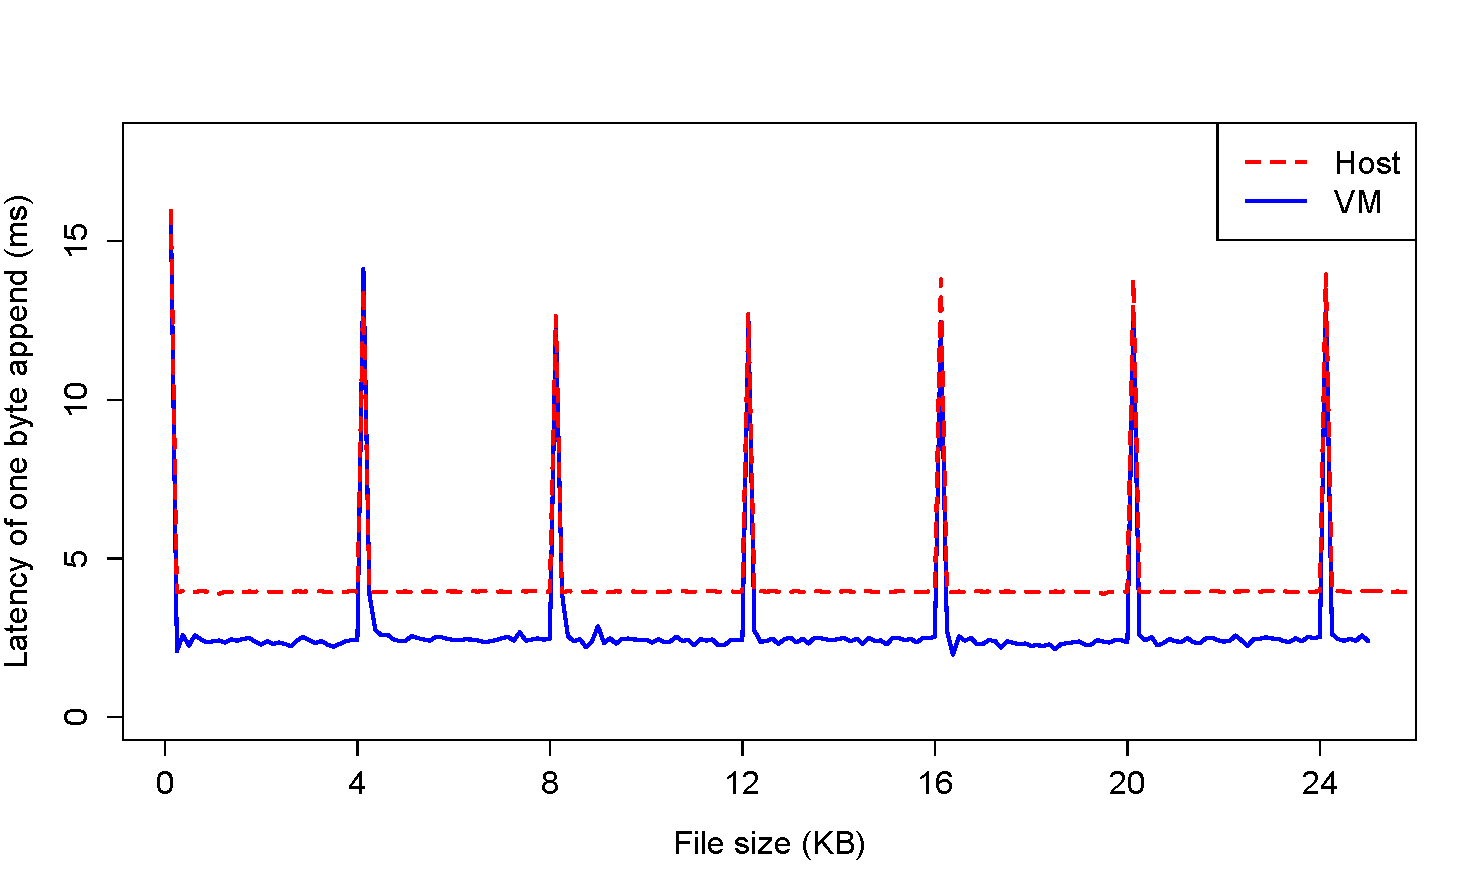
\includegraphics[width=1\textwidth]{./figures/p4_small.pdf}
		\caption{Smaller scale measurements}
		\label{fig:p4smallgraph}
    \end{subfigure}
    \begin{subfigure}[b]{0.5\textwidth}
		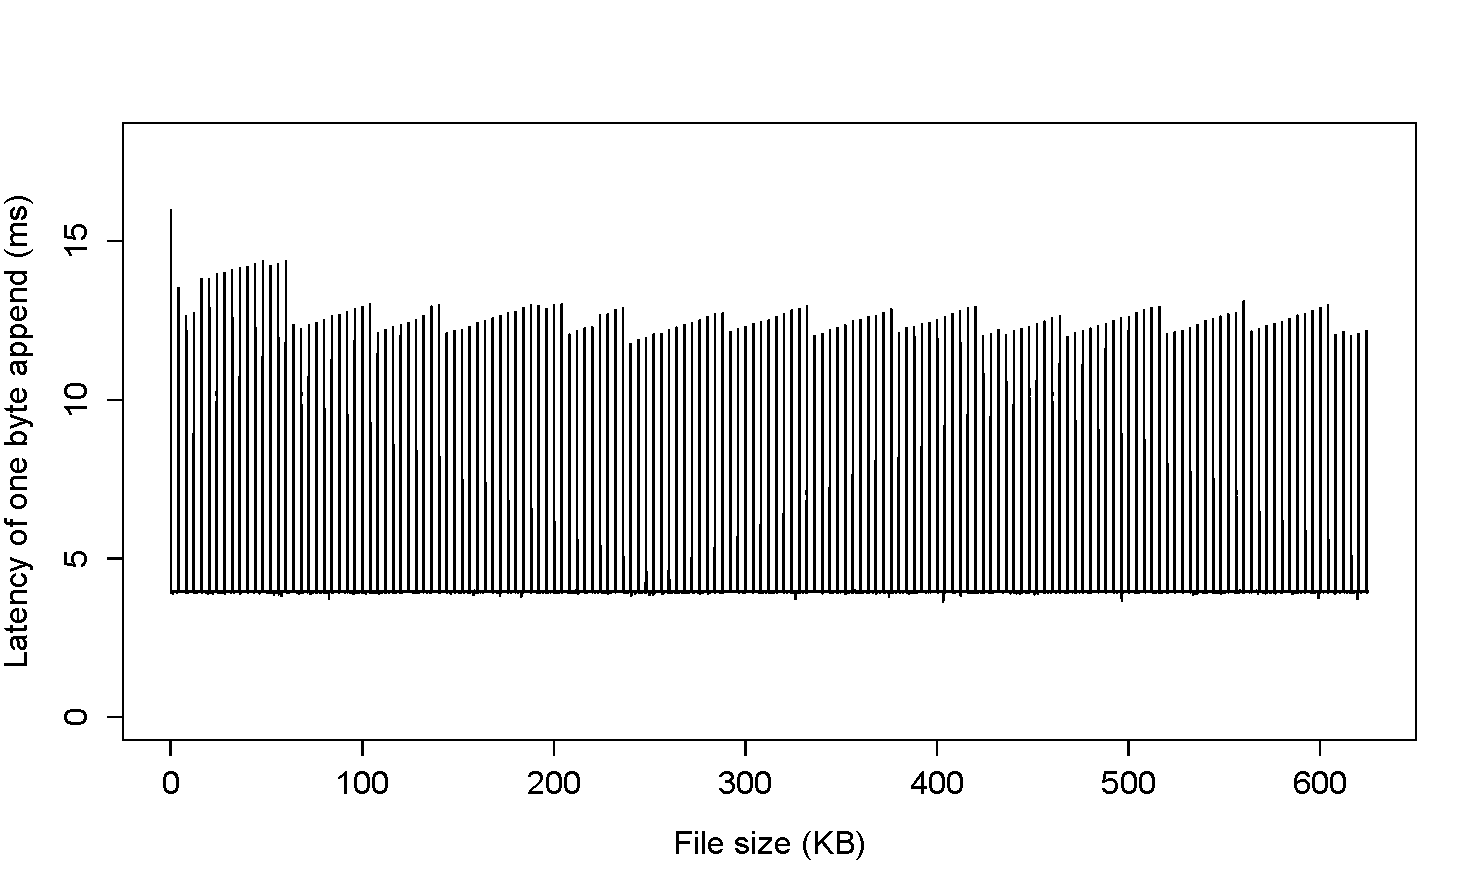
\includegraphics[width=1\textwidth]{./figures/p4_big.pdf}
		\caption{Bigger scale measurements on host}
		\label{fig:p4biggraph}
    \end{subfigure}
	\caption{Latency of one-byte append for varying file sizes. Horizontal axis shows existing file size and vertical axis shows latency of appending one byte to that file.}
	\label{fig:p4}
\end{figure}

\begin{figure}
\begin{algorithmic}
\STATE create a $file$
\STATE $buffer\_size \leftarrow$ 128
\FOR{$i = 0$ to $MAX\_SIZE$}
\STATE $buffer \leftarrow$ random $buffer\_size$ bytes
\STATE start\_timer
\STATE write first byte of $buffer$
\STATE end\_timer and save the result
\STATE write the rest $buffer\_size - 1$ bytes
\ENDFOR
\end{algorithmic}
\caption{Function used to measure one-byte append latency}
\label{fig:p4pseudo}
\end{figure}
